\pagebreak

\appendix

\section{Proofs}\label{sec:proofs}
The definitions of continuity and convergence for pseudo-metrics are similar to those for metrics, and we state them below.

A function $f: \gQ \mapsto \gQ$ is continuous with respect to a pseudo-metric $d$ if for any $p \in \gQ$ and any scalar $\epsilon > 0$, there exists a $\delta$ such that for all \mbox{$q \in \gQ$},
\begin{align*}
    d(p, q) < \delta
    \implies
    d(f(p), f(q)) < \epsilon.
\end{align*}

An infinite sequence $p_1, p_2 \dots$ converges to a value $p$ with respect to a pseudo-metric $d$, which we write as
\begin{align*}
    \limt p_t \rightarrow p,
\end{align*}
if
\begin{align*}
    \limt d(p_t, p) \rightarrow 0.
\end{align*}

Note that if $f$ is continuous, then
\begin{align*}
    \lim_{t \rightarrow \infty} \dent(p_t, q) \rightarrow 0
    \implies
    \lim_{t \rightarrow \infty} \dent(f(p_t), f(q)) \rightarrow 0.
\end{align*}

\subsection{Proof of Lemma 3.1}\label{sec:general-proof}
\begin{lemma}
Let $\Imgs$ be a compact set.
Define the set of distributions $\gQ = \{p : \support(p) \subseteq \Imgs\}$.
Let $\gF: \gQ \mapsto \gQ$ be continuous with respect to the pseudometric \mbox{$\dent(p, q) \triangleq |\gH(p) - \gH(q)|$} and $\gH(\gF(p)) \geq \gH(p)$ with equality if and only if $p$ is the uniform probability distribution on $\Imgs$, denoted as $\U$.
Define the sequence of distributions $P = (p_1, p_2, \dots)$ by starting with any $p_1 \in \gQ$ and recursively defining $p_{t+1} = \gF(p_t)$.
The sequence $P$ converges to $\U$ with respect to $\dent$. In other words, \mbox{$\lim_{t \rightarrow 0} |\gH(p_t) - \gH(\U)| \rightarrow 0$}.
\end{lemma}
\begin{proof}
The idea of the proof is to show that the distance (with respect to $\dent$) between $p_t$ and $\U$ converges to a value.
If this value is $0$, then the proof is complete since $\U$ uniquely has zero distance to itself.
Otherwise, we will show that this implies that $\gF$ is not continuous, which a contradiction.

For shorthand, define $d_t$ to be the $\dent$-distance to the uniform distribution, as in
\begin{align*}
    d_t \triangleq \dent(p_t, \U).
\end{align*}
First we prove that $d_t$ converges.
Since the entropies of the sequence $(p_1, \dots)$ monotonically increase, we have that
\begin{align*}
    d_1 \geq d_2 \geq \dots.
\end{align*}
We also know that $d_t$ is lower bounded by $0$, and so by the monotonic convergence theorem, we have that
\begin{align*}
    \lim_{t\rightarrow\infty} d_t \rightarrow d^*.
\end{align*}
for some value $d^* \geq 0$.

To prove the lemma, we want to show that $d^* = 0$.
Suppose, for contradiction, that $d^* \neq 0$.
Then consider any distribution, $q^*$, such that $\dent(q^*, \U) = d^*$.
Such a distribution always exists since we can continuously interpolate entropy values between $\gH(p_1)$ and $\gH(\U)$ with a mixture distribution.
Note that $q^* \neq \U$ since \mbox{$\dent(\U, \U) = 0$}.
Since \mbox{$\limt d_t \rightarrow d^*$}, we have that
\begin{align}\label{eq:dent-distance-goes-to-zero}
    \limt
    \dent(p_t, q^*) \rightarrow 0,
\end{align}
and so
\begin{align*}
    \limt p_t \rightarrow q^*.
\end{align*}
Because the function $\gF$ is continuous with respect to $\dent$, \autoref{eq:dent-distance-goes-to-zero} implies that
\begin{align*}
    \limt
    \dent(\gF(p_t), \gF(q^*)) \rightarrow 0.
\end{align*}
However, since $\gF(p_t) = p_{t+1}$ we can equivalently write the above equation as
\begin{align*}
    \limt
    \dent(p_{t+1}, \gF(q^*)) \rightarrow 0.
\end{align*}
which, through a change of index variables, implies that
\begin{align*}
    \limt
    p_t \rightarrow \gF(q^*)
\end{align*}
Since $q^*$ is not the uniform distribution, we have that \mbox{$\gH(\gF(q^*)) > \gH(q^*)$}, which implies that $\gF(q^*)$ and $q^*$ are unique distributions.
So, $p_t$ converges to two distinct values, $q^*$ and $\gF(q^*)$, which is a contradiction.
Thus, it must be the case that $d^* = 0$, completing the proof.
\end{proof}

%-------------------------------------------------
%-------------------------------------------------
%-------------------------------------------------
\subsection{Proof of Lemma 3.2}\label{sec:covariance-proof}
\begin{lemma}\label{lemma:covariance-general}
Given two distribution $p(x)$ and $q(x)$ where $p \ll q$ and
\begin{align}
   0 < \Cov_p[\log p(X), \log q(X)]
\end{align}
define the distribution $p_\alpha$ as
\begin{align*}
    p_\alpha(x) &= \frac{1}{Z_\alpha} p(x) q(x)^\alpha
\end{align*}
where $\alpha \in \R$ and $Z_\alpha$ is the normalizing factor.
Let $\gH_\alpha(\alpha)$ be the entropy of $p_\alpha$.
Then there exists a constant $a > 0$ such that for all $\alpha \in [-a, 0)$,
\begin{align}
    \gH_\alpha(\alpha) > \gH_\alpha(0) = \gH(p).
\end{align}

\end{lemma}
\begin{proof}
Observe that $\{p_\alpha : \alpha \in [-1, 0]\}$ is a one-dimensional exponential family
\begin{align*}
    p_\alpha(x) = e^{\alpha T(x) - A(\alpha) + k(x)}
\end{align*}
with log carrier density $k(x) = \log p(x)$, natural parameter $\alpha$, sufficient statistic $T(x) = \log q(x)$, and log-normalizer $A(\alpha) = \int_{\gX} e^{\alpha T(x) + k(x)}dx$.
As shown in \cite{nielsen2010entropies}, the entropy of a distribution from a one-dimensional exponential family with parameter $\alpha$ is given by:
\begin{align*}
    \gH_\alpha(\alpha) \triangleq
    \gH(p_\alpha)
    = A(\alpha) - \alpha A'(\alpha) - \E_{p_\alpha}[k(X)]
\end{align*}
The derivative with respect to $\alpha$ is then
\begin{align*}
    \frac{d}{d \alpha}\gH_\alpha(\alpha)
        &= - \alpha A''(\alpha) - \frac{d}{d\alpha}\E_{p_\alpha}[k(x)]\\
        &= - \alpha A''(\alpha) - \E_\alpha[k(x)(T(x) - A'(\alpha)]\\
        &= - \alpha \Var_{p_\alpha}[T(x)] - \Cov_{p_\alpha}[k(x), T(x)]
\end{align*}
where we use the fact that the $n$th derivative of $A(\alpha)$ give the $n$ central moment, i.e. $A'(\alpha) = \E_{p_\alpha}[T(x)]$ and $A''(\alpha) = \Var_{p_\alpha}[T(x)]$.
The derivative of $\alpha = 0$ is
\begin{align*}
    \frac{d}{d \alpha}\gH_\alpha(0)
        &= - \Cov_{p_0}[k(x), T(x)]\\
        &= - \Cov_p[\log p(x), \log q(x)]
\end{align*}
which is negative by assumption.
Because the derivative at $\alpha = 0$ is negative, then there exists a constant $a > 0$ such that for all $\alpha \in [-a, 0]$, $\gH_\alpha(\alpha) > \gH_\alpha(0) = \gH(p)$.
\end{proof}
The paper applies \label{lemma:covariance-general} to the case where $q = \pg$ and $p=\pstate$.
When we take $N \rightarrow \infty$, we have that $\pskewed$ corresponds to $p_\alpha$ above.

%-------------------------------------------------
%-------------------------------------------------
%-------------------------------------------------
\subsection{Simple Case Proof}\label{sec:simple-case-proof}
We prove the convergence directly for the (even more) simplified case when $\papprox = \pspgt$ using a similar technique:
\begin{lemma}\label{lemma:all-equal}
Assume the set $\Imgs$ has finite volume so that its uniform distribution $\U$ is well defined and has finite entropy.
Given any distribution $p(\st)$ whose support is $\Imgs$, recursively define $p_t$ with $p_1 = p$ and
\begin{align*}
    p_{t+1}(\st)
        &= \frac{1}{Z_\alpha^t} p_t(\st)^{\alpha}, \quad \forall \st \in \Imgs
\end{align*}
where $Z_\alpha^t$ is the normalizing constant and $\alpha \in [0, 1)$.

The sequence $(p_1, p_2, \dots)$ converges to $\U$, the uniform distribution $\Imgs$.
\end{lemma}
\begin{proof}
If $\alpha = 0$, then $p_2$ (and all subsequent distributions) will clearly be the uniform distribution.
We now study the case where $\alpha \in (0, 1)$.

At each iteration $t$, define the one-dimensional exponential family $\{\ptt : \theta \in [0, 1]\}$ where $\ptt$ is
\begin{align*}
    \ptt(\st) = e^{\theta T(\st) - A(\theta) + k(\st)}
\end{align*}
with log carrier density $k(\st) = 0$, natural parameter $\theta$, sufficient statistic $T(\st) = \log p_t(\st)$, and log-normalizer $A(\theta) = \int_{\Imgs} e^{\theta T(\st)} d\st$.
As shown in \cite{nielsen2010entropies}, the entropy of a distribution from a one-dimensional exponential family with parameter $\theta$ is given by:
\begin{align*}
    \htt(\theta) \triangleq \gH(\ptt) = A(\theta) - \theta A'(\theta)
\end{align*}
The derivative with respect to $\theta$ is then
\begin{align}\nonumber
    \frac{d}{d \theta}d\htt(\theta)
        &= - \theta A''(\theta)\\\nonumber
        &= - \theta \Var_{\st \sim \ptt}[T(\st)]\\\label{eq:easy-variance-case}
        &= - \theta \Var_{\st \sim \ptt}[\log p_t(\st)]\\\nonumber
        &\leq 0
\end{align}
where we use the fact that the $n$th derivative of $A(\theta)$ is the $n$ central moment, i.e. $A''(\theta) = \Var_{\st \sim \ptt}[T(\st)]$.
Since variance is always non-negative, this means the entropy is monotonically decreasing with $\theta$.
Note that $p_{t+1}$ is a member of this exponential family, with parameter $\theta = \alpha \in (0, 1)$.
So
\begin{align*}
    \gH(p_{t+1}) = \htt(\alpha) \geq \htt(1) = \gH(p_t)
\end{align*}
which implies
\begin{align*}
    \gH(p_1) \leq \gH(p_2) \leq \dots.
\end{align*}
This monotonically increasing sequence is upper bounded by the entropy of the uniform distribution, and so this sequence must converge.

The sequence can only converge if $\frac{d}{d \theta} \htt(\theta)$ converges to zero.
However, because $\alpha$ is bounded away from $0$, \Eqref{eq:easy-variance-case} states that this can only happen if
\begin{align}\label{eq:easy-logprob-becomes-constant}
    \Var_{\st \sim \ptt}[\log p_t(\st)] \rightarrow 0.
\end{align}
Because $p_t$ has full support, then so does $\ptt$.
Thus, \Eqref{eq:easy-logprob-becomes-constant} is only true if $\log p_t(\st)$ converges to a constant, i.e. $p_t$ converges to the uniform distribution.
\end{proof}

%-------------------------------------------------
%-------------------------------------------------
%-------------------------------------------------


\section{Additional Experiments}\label{sec:add-exps}

\subsection{Sensitivity Analysis}\label{sensitivity}
\paragraph{Sensitivity to RL Algorithm}
In our experiments, we combined \METHOD with soft actor critic (SAC)~\citep{haarnoja2018sacapp}.
We conduct a set of experiments to test whether \METHOD may be used with other RL algorithms for training the goal-conditioned policy.
To that end, we replaced SAC with twin delayed deep deterministic policy gradient (TD3)~\citep{fujimoto2018td3} and ran the same \METHOD experiments on Visual Door, Visual Pusher, and Visual Pickup.
In \autoref{fig:rl-sweep}, we see that \METHOD performs consistently well with both SAC and TD3, demonstrating that \METHOD is beneficial across multiple RL algorithms.
\begin{figure}
    \begin{subfigure}{\linewidth}
      \centering
      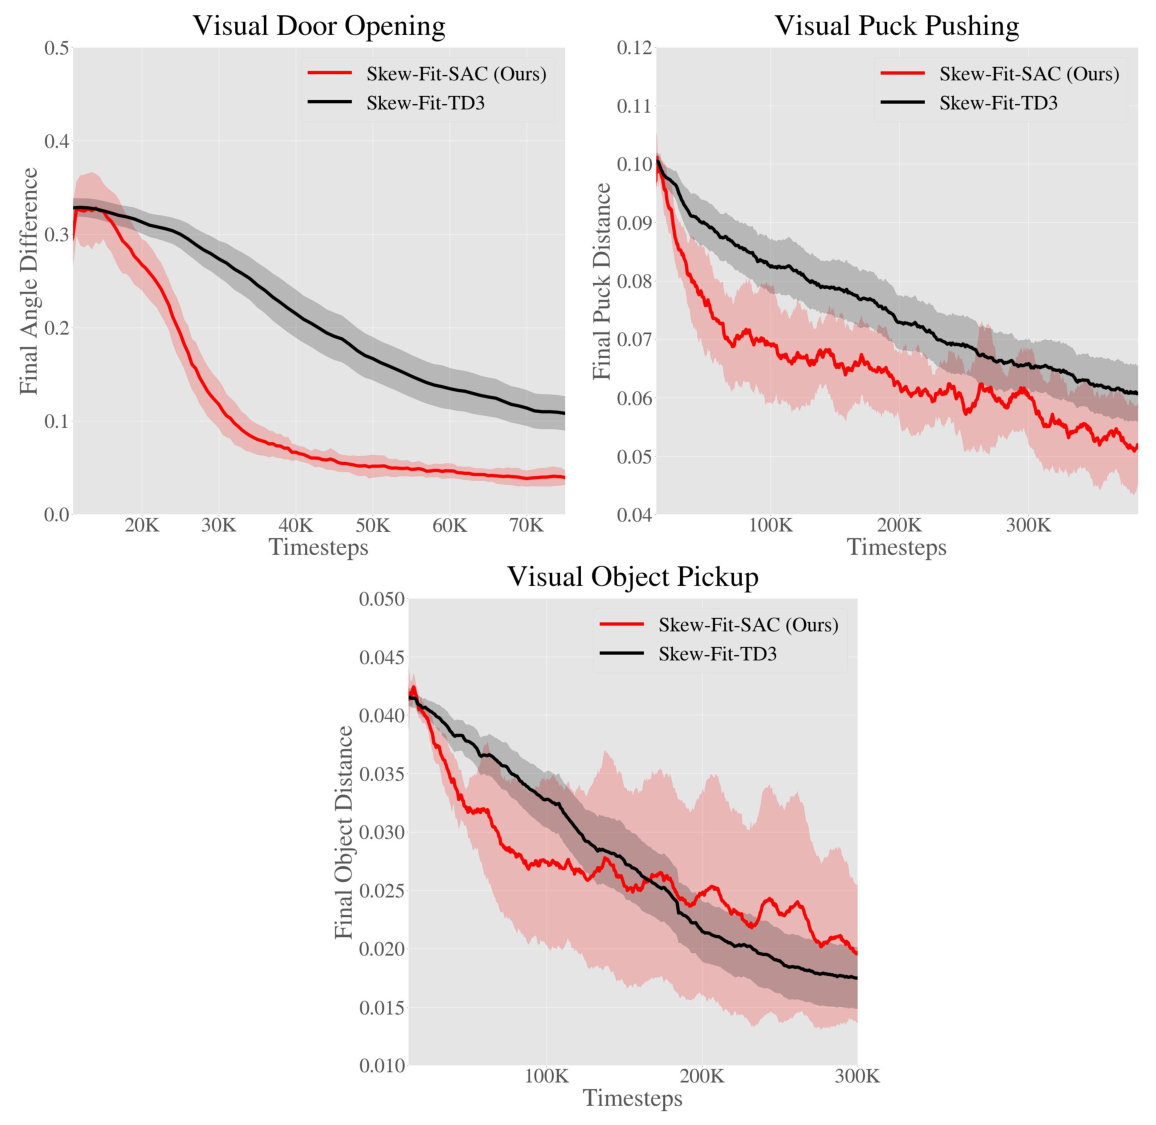
\includegraphics[width=\linewidth]{figures/plots/td3vskewfit.pdf}
      \label{fig:door-rl-sweep}
    \end{subfigure}
    \\
  \vspace{-.1in}
  \fcaption{
  We compare using SAC~\citep{haarnoja2018sacapp} and TD3~\citep{fujimoto2018td3} as the underlying RL algorithm on Visual Door, Visual Pusher and Visual Pickup.
  We see that \METHOD works consistently well with both SAC and TD3, demonstrating that \METHOD may be used with various RL algorithms.
  For the experiments presented in \autoref{sec:experiments}, we used SAC.
  }
  \vspace{-0.05 cm}
  \label{fig:rl-sweep}
\end{figure}

\paragraph{Sensitivity to $\alpha$ Hyperparameter}
We study the sensitivity of the $\alpha$ hyperparameter by testing values of \mbox{$\alpha \in [-1, -0.75, -0.5, -0.25, 0]$} on the Visual Door and Visual Pusher task.
The results are included in \Figref{fig:alpha-sweep} and shows that our method is  robust to different parameters of $\alpha$, particularly for the more challenging Visual Pusher task.
Also, the method consistently outperform $\alpha=0$, which is equivalent to sampling uniformly from the replay buffer.
\begin{figure}[!ht]
  \centering
  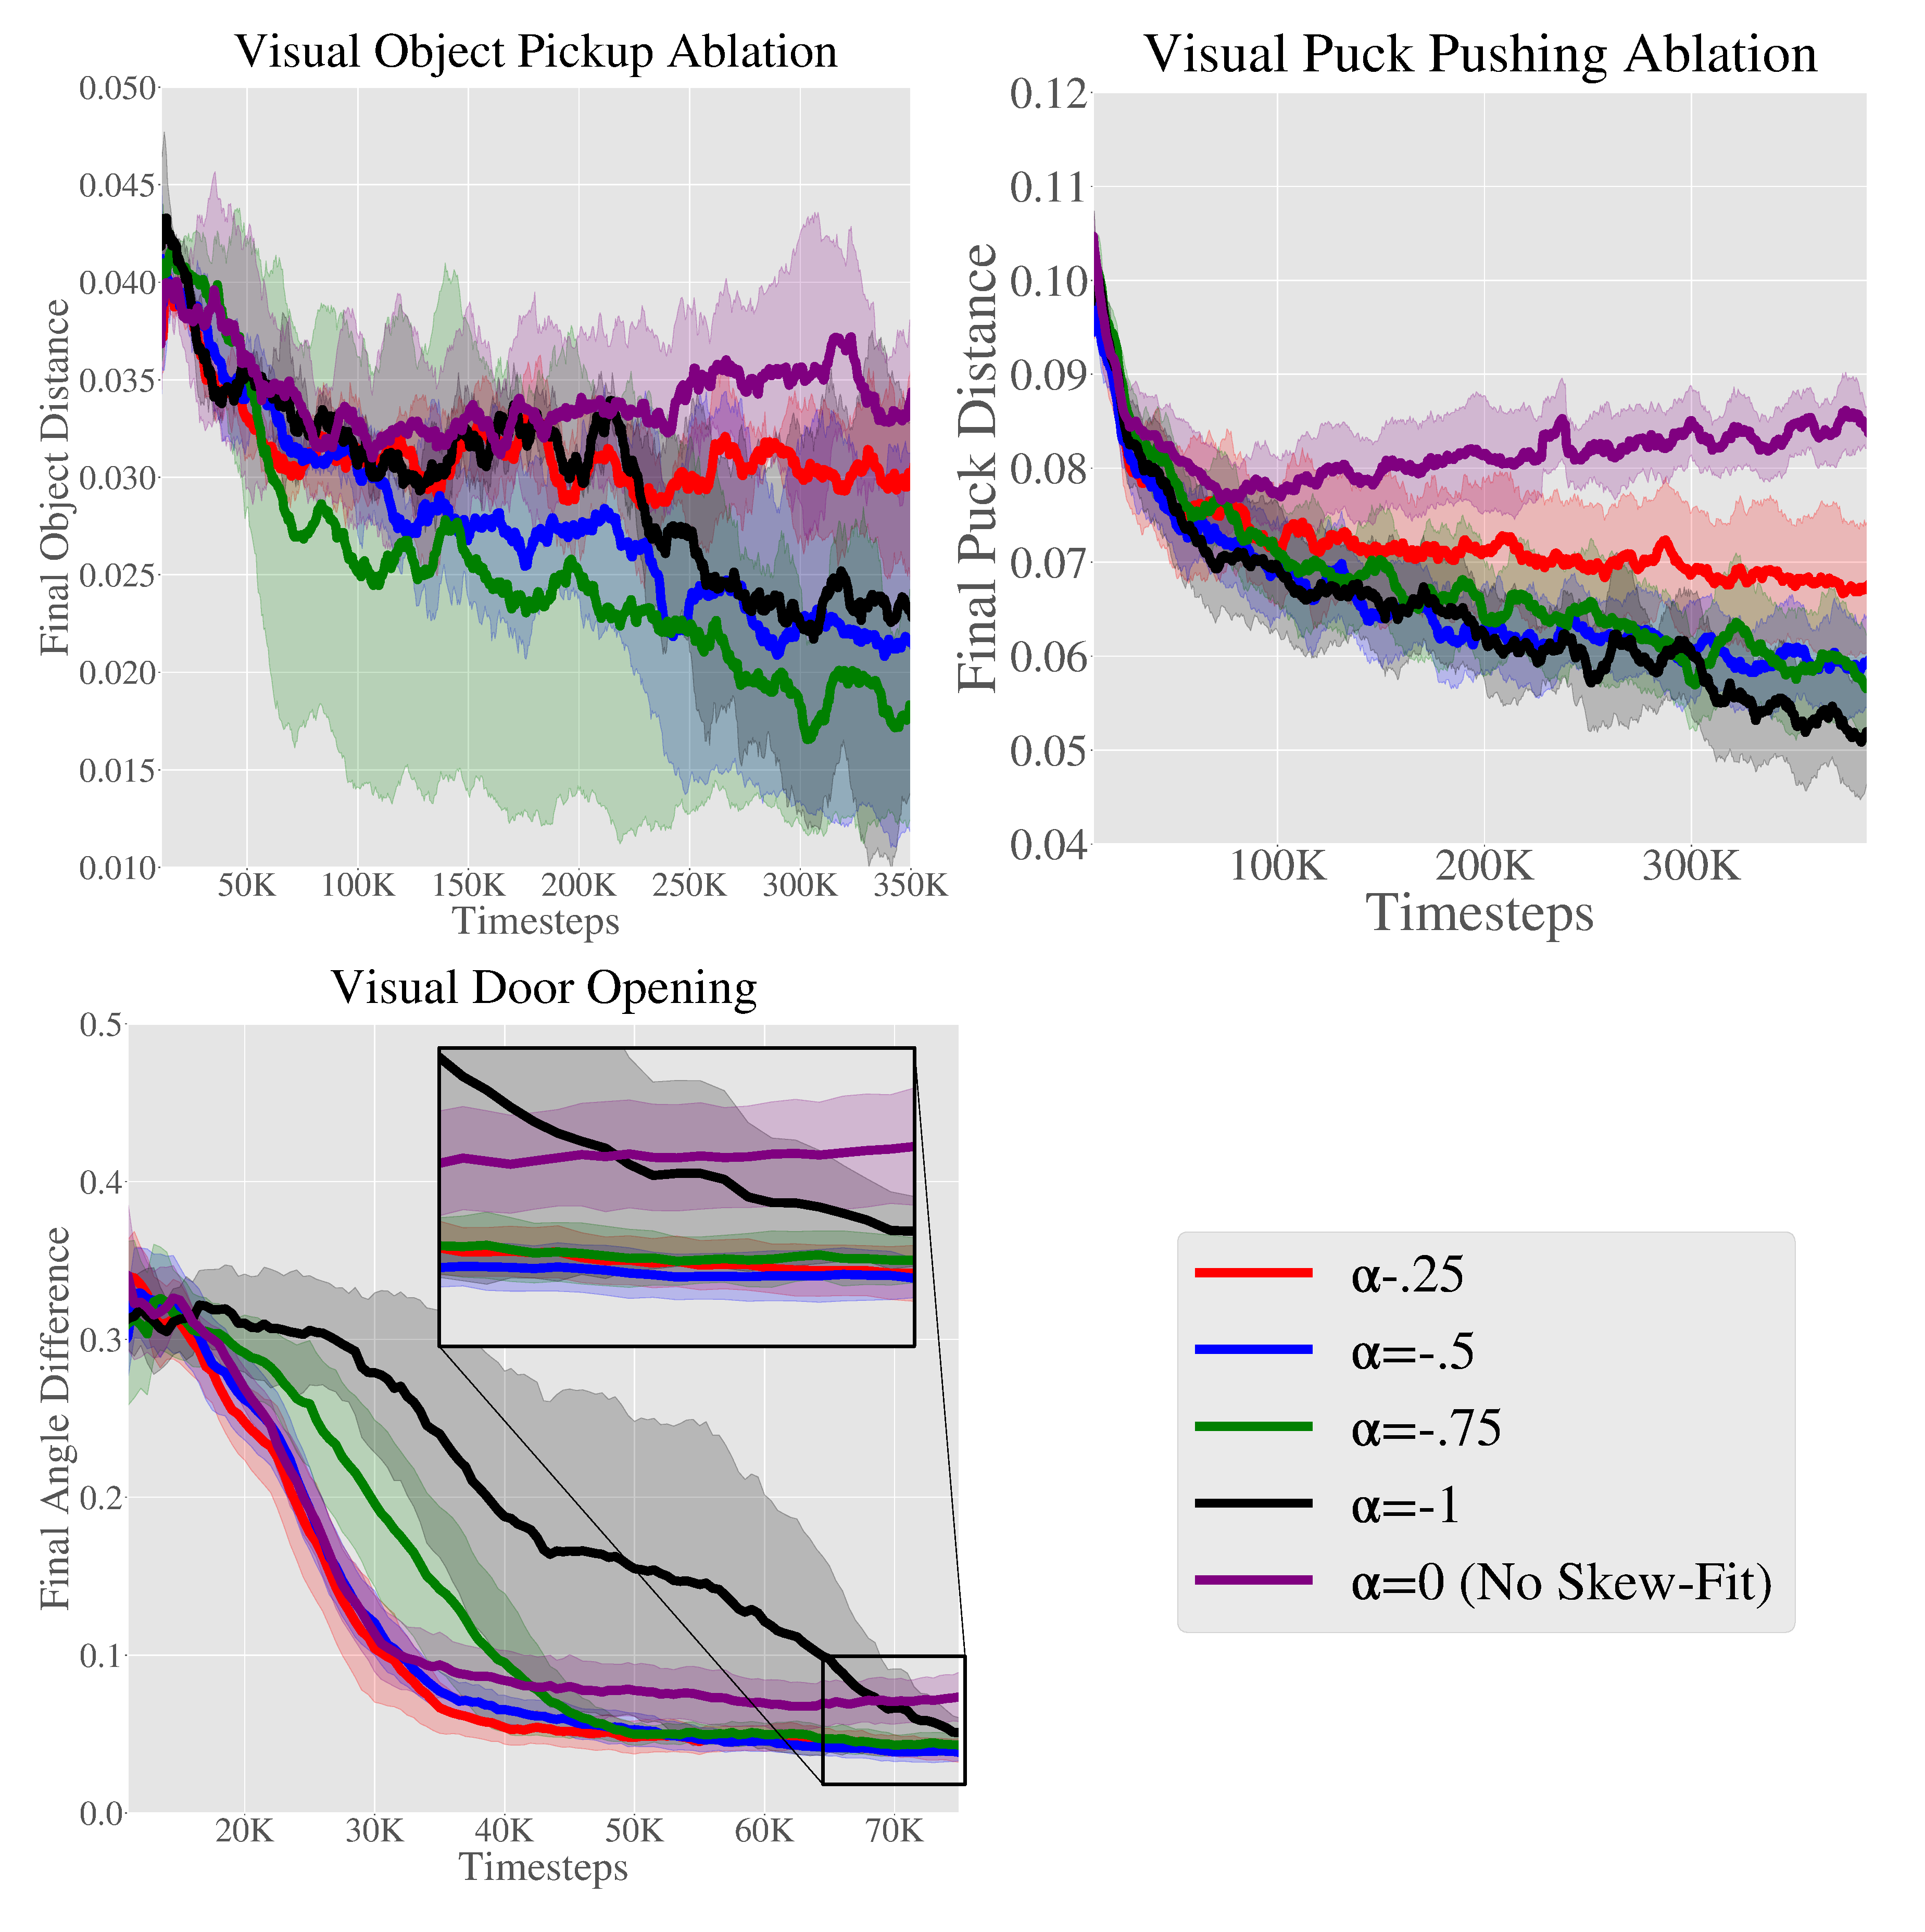
\includegraphics[width=1\linewidth]{figures/plots/power_ablation_square_with_inset.pdf}
  \vspace{-.05in}
  \label{fig:door-alpha-sweep}
  \vspace{-.1in}
  \fcaption{
  We sweep different values of $\alpha$ on Visual Door, Visual Pusher and Visual Pickup.
  \METHOD helps the final performance on the Visual Door task, and outperforms No Skew-Fit ($\alpha=0$) as seen in the zoomed in version of the plot.
  In the more challenging Visual Pusher task, we see that \METHOD consistently helps and halves the final distance.
  Similarly, we observe that \METHOD consistently outperforms No Skew-fit on Visual Pickup.
  Note that alpha=-1 is not always the optimal setting for each environment, but outperforms $\alpha=0$ in each case in terms of final performance.
  }
  \vspace{-0.05 cm}
  \label{fig:alpha-sweep}
\end{figure}

 \subsection{Variance Ablation} \label{sec:analysis-variance}
 \begin{figure}[H]
     \vspace{0.1in}
         \centering
         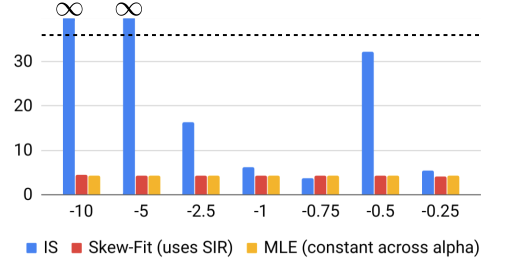
\includegraphics[width=0.8\linewidth]{figures/plots/variance.png}
         \fcaption{Gradient variance averaged across parameters in last epoch of training VAEs. Values of $\alpha$ less than $-1$ are numerically unstable for importance sampling (IS), but not for Skew-Fit.}
         \label{fig:grad-var}
     \label{fig:ul-variance-results}
 \end{figure}
We measure the gradient variance of training a VAE on an unbalanced Visual Door image dataset with \METHOD vs \METHOD with importance sampling (IS) vs no \METHOD (labeled MLE). We construct the imbalanced dataset by rolling out a random policy in the environment and collecting the visual observations. Most of the images contained the door in a closed position; in a few, the door was opened.
 In \autoref{fig:ul-variance-results}, we see that the gradient variance for Skew-Fit with IS is catastrophically large for large values of $\alpha$.
 In contrast, for Skew-Fit with SIR, which is what we use in practice, the variance is relatively similar to that of MLE. Additionally we trained three VAE's, one with MLE on a uniform dataset of valid door opening images, one with Skew-Fit on the unbalanced dataset from above, and one with MLE on the same unbalanced dataset. As expected, the VAE that has access to the uniform dataset gets the lowest negative log likelihood score.
 This is the oracle method, since in practice we would only have access to imbalanced data.
 As shown in \autoref{table:ll-ablation}, \METHOD considerably outperforms MLE, getting a much closer to oracle log likelihood score.
 \begin{table}
         \centering
         \begin{tabular}{|l|l|}
         \hline
             {\footnotesize \textbf{Method}}                 & {\footnotesize \textbf{NLL}}   \\\hline
             {\footnotesize MLE on uniform (oracle)} & {\footnotesize 20175.4}               \\\hline
             {\footnotesize Skew-Fit on unbalanced}           & {\footnotesize 20175.9}              \\\hline
             {\footnotesize MLE on unbalanced}                    & {\footnotesize 20178.03} \\\hline
         \end{tabular}
         \fcaption{Despite training on a unbalanced Visual Door dataset (see Figure 7 of paper), the negative log-likelihood (NLL) of Skew-Fit evaluated on a uniform dataset matches that of a VAE trained on a uniform dataset.}
         \label{table:ll-ablation}
 \end{table}


\subsection{Goal and Performance Visualization}\label{sec:vae-dump}
We visualize the goals sampled from \METHOD as well as those sampled when using the prior method, RIG~\citep{nair2018rig}.
As shown in \autoref{fig:vae_dump} and \autoref{fig:vae_dump_real}, the generative model $\pg$ results in much more diverse samples when trained with \METHOD.
We we see in \autoref{fig:example_rollouts}, this results in a policy that more consistently reaches the goal image.
\begin{figure*}
    \centering
    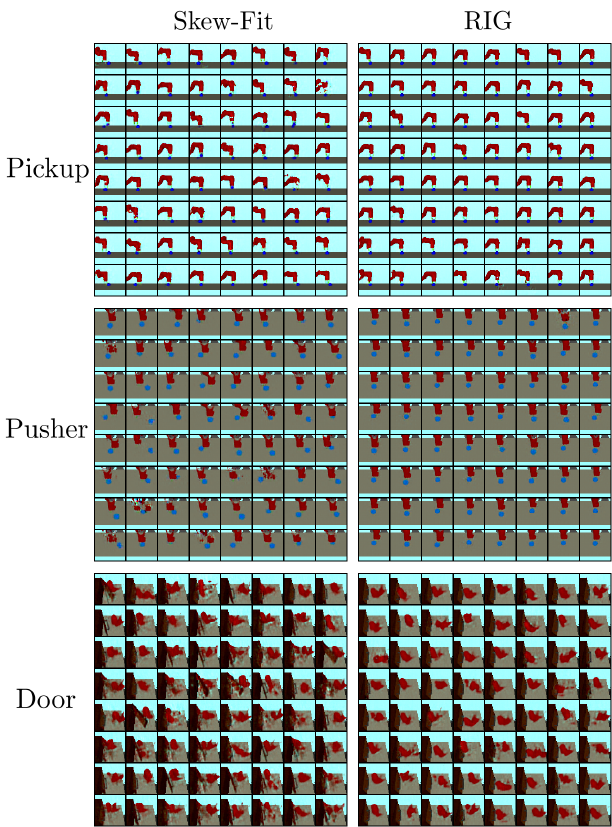
\includegraphics[width=0.9\textwidth]{figures/vae_samples_v3-01.png}
    \fcaption{
Proposed goals from the VAE for RIG and with \METHOD on the \textit{Visual Pickup}, \textit{Visual Pusher}, and \textit{Visual Door} environments. Standard RIG produces goals where the door is closed and the object and puck is in the same position, while RIG + \METHOD proposes goals with varied puck positions, occasional object goals in the air, and both open and closed door angles.
    }
    \label{fig:vae_dump}
\end{figure*}

\begin{figure*}
    \centering
    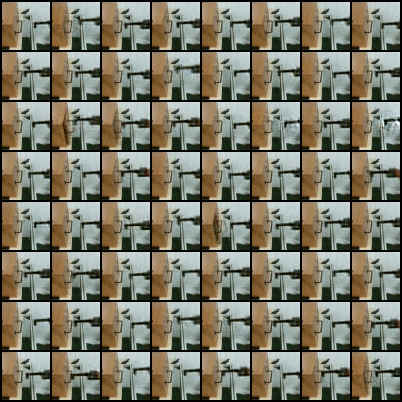
\includegraphics[width=0.25\textheight]{figures/vae_dumps/rig-real-world-v2-exp-samples.png}
    \hspace{.3 in}
    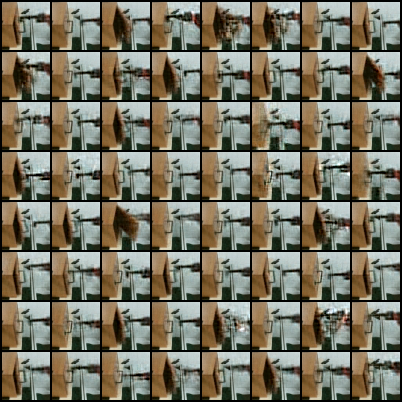
\includegraphics[width=0.25\textheight]{figures/vae_dumps/skew-fit-real-world-v2-exp-samples.png}
    \fcaption{
Proposed goals from the VAE for RIG (left) and with RIG + \METHOD (right) on the \textit{Real World Visual Door} environment. Standard RIG produces goals where the door is closed  while RIG + \METHOD proposes goals with both open and closed door angles.
    }
    \label{fig:vae_dump_real}
\end{figure*}
\begin{figure*}
    \centering
    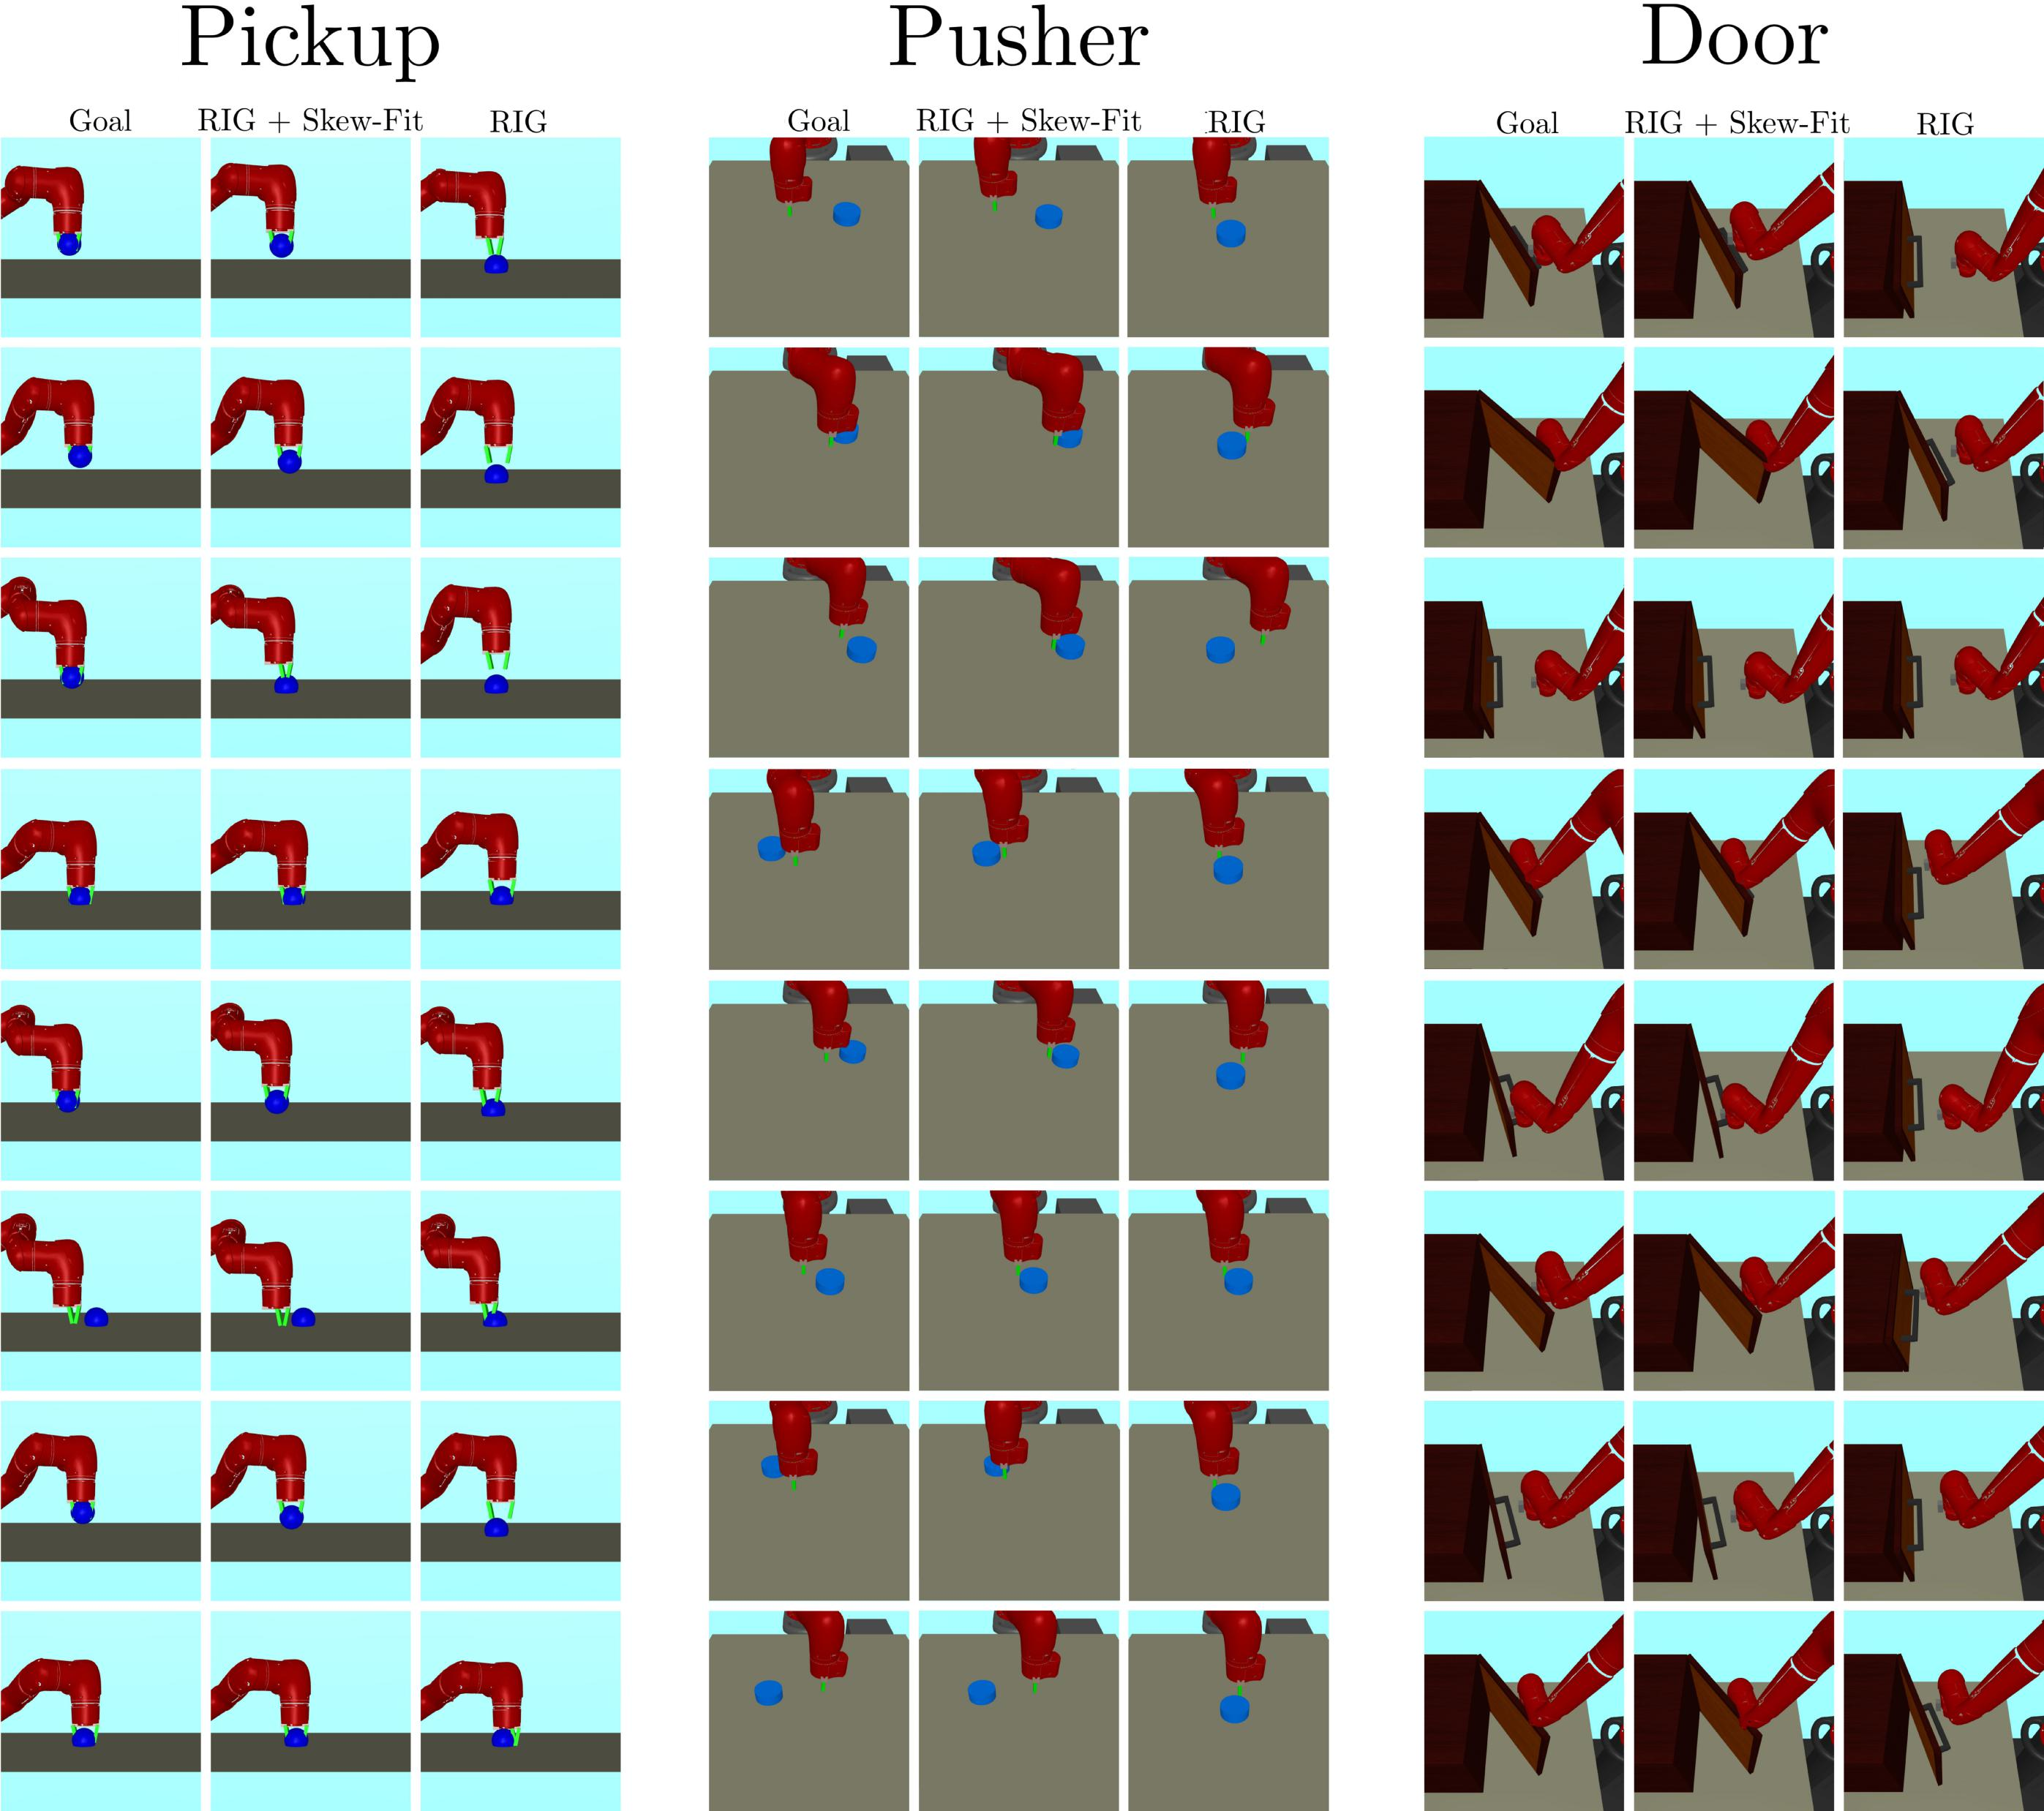
\includegraphics[width=0.9\textwidth]{figures/example-rollouts.jpg}
    \fcaption{
Example reached goals by \METHOD and RIG. The first column of each environment section specifies the target goal while the second and third columns show reached goals by \METHOD and RIG. Both methods learn how to reach goals close to the initial position, but only \METHOD learns to reach the more difficult goals.
    }
    \label{fig:example_rollouts}
\end{figure*}

\section{Implementation Details}\label{sec:implementation-details}

\subsection{Likelihood Estimation using $\beta$-VAE}\label{sec:likelihood-estimation-vae}
We estimate the density under the VAE by using a sample-wise approximation to the marginal over $x$ estimated using importance sampling:
\begin{align*}
    \pgt(x) &= \mathbb E_{z \sim q_{\theta_t}(z|x)} \left[\frac{p(z)}{q_{\theta_t}(z|x)} p_{\psi_t}(x \mid z) \right]  \\
    &\approx \frac{1}{N} \sum_{i=1}^{N} \left[\frac{p(z)}{q_{\theta_t}(z|x)} p_{\psi_t}(x \mid z) \right].
\end{align*}
where $q_{\theta}$ is the encoder, $p_\psi$ is the decoder, and $p(z)$ is the prior, which in this case is unit Gaussian.
We found that sampling $N=10$ latents for estimating the density worked well in practice.

\subsection{Oracle 2D Navigation Experiments}\label{sec:2d-details}
We initialize the VAE to the bottom left corner of the environment for \textit{Four Rooms}.
Both the encoder and decoder have 2 hidden layers with [400, 300] units,  ReLU hidden activations, and no output activations.
The VAE has a latent dimension of $8$ and a Gaussian decoder trained with a fixed variance, batch size of $256$, and $1000$ batches at each iteration. The VAE is trained on the exploration data buffer every 1000 rollouts.

\subsection{Implementation of SAC and Prior Work}\label{sec:prior-work-implementation}
For all experiments, we trained the goal-conditioned policy using soft actor critic (SAC)~\citep{haarnoja2018sacapp}.
To make the method goal-conditioned, we concatenate the target XY-goal to the state vector.
During training, we retroactively relabel the goals~\citep{kaelbling1993goals,andrychowicz2017her} by sampling from the goal distribution with probabilty $0.5$.
Note that the original RIG~\cite{nair2018rig} paper used TD3~\cite{fujimoto2018td3}, which we also replaced with SAC in our implementation of RIG.
We found that maximum entropy policies in general improved the performance of RIG, and that we did not need to add noise on top of the stochastic policy's noise.
In the prior RIG method, the VAE was pre-trained on a uniform sampling of images from the state space of each environment.
In order to ensure a fair comparison to Skew-Fit, we forego pre-training and instead train the VAE alongside RL, using the variant described in the RIG paper.
For our RL network architectures and training scheme, we use fully connected networks for the policy, Q-function and value networks with two hidden layers of size $400$ and $300$ each.
We also delay training any of these networks for $10000$ time steps in order to collect sufficient data for the replay buffer as well as to ensure the latent space of the VAE is relatively stable (since we continuously train the VAE concurrently with RL training).
As in RIG, we train a goal-conditioned value functions~\cite{schaul2015uva} using hindsight experience replay~\cite{andrychowicz2017her}, relabelling $50\%$ of exploration goals as goals sampled from the VAE prior $\mathcal{N} (0, 1)$ and $30\%$ from future goals in the trajectory.

For our implementation of \citep{hazan2019provably}, we trained the policies with the reward
\begin{align*}
    r(s) = r_\text{Skew-Fit}(s) + \lambda \cdot r_\text{Hazan et al.}(s)
\end{align*}

For $r_\text{Hazan et al.}$, we use the reward described in Section 5.2 of \citet{hazan2019provably}, which requires an estimated likelihood of the state.
To compute these likelihood, we use the same method as in Skew-Fit (see \autoref{sec:likelihood-estimation-vae}).
With 3 seeds each, we tuned $\lambda$ across values $[100, 10, 1, 0.1, 0.01, 0.001]$ for the door task, but all values performed poorly.
For the pushing and picking tasks, we tested values across $[1, 0.1, 0.01, 0.001, 0.0001]$ and found that 0.1 and 0.01 performed best for each task, respectively.

\subsection{RIG with \METHOD Summary}\label{sec:rig-and-full-method}
\autoref{alg:rig-and-full-method-details} provides detailed pseudo-code for how we combined our method with RIG.
Steps that were removed from the base RIG algorithm are highlighted in blue and steps that were added are highlighted in red.
The main differences between the two are (1) not needing to pre-train the $\beta$-VAE, (2) sampling exploration goals from the buffer using $\pskewed$ instead of the VAE prior, (3) relabeling with replay buffer goals sampled using $\pskewed$ instead of from the VAE prior, and (4) training the VAE on replay buffer data data sampled using $\pskewed$ instead of uniformly.

\subsection{Vision-Based Continuous Control Experiments}\label{sec:vision-based-appendix}
In our experiments, we use an image size of 48x48.
For our VAE architecture, we use a modified version of the architecture used in the original RIG paper ~\cite{nair2018rig}.
Our VAE has three convolutional layers with kernel sizes: 5x5, 3x3, and 3x3, number of output filters: 16, 32, and 64 and strides: 3, 2, and 2.
We then have a fully connected layer with the latent dimension number of units, and then reverse the architecture with de-convolution layers.
We vary the latent dimension of the VAE, the $\beta$ term of the VAE and the $\alpha$ term for \METHOD based on the environment.
Additionally, we vary the training schedule of the VAE based on the environment. See the table at the end of the appendix for more details.
Our VAE has a Gaussian decoder with identity variance, meaning that we train the decoder with a mean-squared error loss.

When training the VAE alongside RL, we found the following three schedules to be effective for different environments:

\begin{enumerate}
    \item For first $5K$ steps: Train VAE using standard MLE training every $500$ time steps for $1000$ batches. After that, train VAE using \METHOD every $500$ time steps for $200$ batches.
    \item For first $5K$ steps: Train VAE using standard MLE training every $500$ time steps for $1000$ batches. For the next $45K$ steps, train VAE using \METHOD every $500$ steps for $200$ batches. After that, train VAE using \METHOD every $1000$ time steps for $200$ batches.
    \item For first $40K$ steps: Train VAE using standard MLE training every $4000$ time steps for $1000$ batches. Afterwards, train VAE using \METHOD every $4000$ time steps for $200$ batches.
\end{enumerate}

We found that initially training the VAE without \METHOD improved the stability of the algorithm.
This is due to the fact that density estimates under the VAE are constantly changing and inaccurate during the early phases of training. Therefore, it made little sense to use those estimates to prioritize goals early on in training.
Instead, we simply train using MLE training for the first $5K$ timesteps, and after that we perform \METHOD according to the VAE schedules above. Table \ref{table:general-hyperparams} lists the hyper-parameters that were shared across the continuous control experiments. Table \ref{table:env-hyperparams} lists hyper-parameters specific to each environment. Additionally, \autoref{sec:rig-and-full-method} discusses the combined RIG + Skew-Fit algorithm.

\begin{table*}
    \centering
    \begin{tabular}{c|c|c}
    \hline
    \textbf{Hyper-parameter} & \textbf{Value} & \textbf{Comments}\\
    \hline
    \# training batches per time step & $2$ & Marginal improvements after $2$\\
    Exploration Noise & None (SAC policy is stochastic) & Did not tune\\
    RL Batch Size & $1024$ & smaller batch sizes work as well\\
    VAE Batch Size &  $64$ & Did not tune \\
    Discount Factor & $0.99$ & Did not tune\\
    Reward Scaling & $1$ & Did not tune\\
    Policy Hidden Sizes & $[400, 300]$ & Did not tune\\
    Policy Hidden Activation & ReLU & Did not tune\\
    Q-Function Hidden Sizes & $[400, 300]$ & Did not tune\\
    Q-Function Hidden Activation & ReLU & Did not tune\\
    Replay Buffer Size & $100000$ & Did not tune\\
    Number of Latents for Estimating Density ($N$) & $10$ & Marginal improvements beyond $10$\\
    \hline
    \end{tabular}
\fcaption{General hyper-parameters used for all \textit{visual} experiments.}
\label{table:general-hyperparams}
\end{table*}



\begin{table*}
    \centering
    \begin{tabular}{c|c|c|c|c}
    \hline
    \textbf{Hyper-parameter} & \textbf{Visual Pusher} & \textbf{Visual Door} & \textbf{Visual Pickup} & \textbf{Real World Visual Door}\\
    \hline
    Path Length & $50$& $100$ & $50$ & $100$ \\
    $\beta$ for $\beta$-VAE & $20$ & $20$ & $30$ & $60$ \\
    Latent Dimension Size & $4$ & $16$ & $16$ & $16$ \\
    $\alpha$ for Skew-Fit & $-1$ & $-1/2$ & $-1$ & $-1/2$ \\
    VAE Training Schedule & $2$ & $1$ & $2$ & $1$ \\
    Sample Goals From & $\pg$ & $\pskewed$ & $\pskewed$ & $\pskewed$ \\
    \hline
    \end{tabular}
\fcaption{Environment specific hyper-parameters for the \textit{visual} experiments}
\label{table:env-hyperparams}
\end{table*}

\begin{table*}
    \centering
    \begin{tabular}{c|c}
    \hline
    \textbf{Hyper-parameter} & \textbf{Value} \\
    \hline
    \# training batches per time step & $.25$\\
    Exploration Noise & None (SAC policy is stochastic) \\
    RL Batch Size & $512$\\
    VAE Batch Size &  $64$\\
    Discount Factor & $\frac{299}{300}$\\
    Reward Scaling & $10$\\
    Path length & $300$\\
    Policy Hidden Sizes & $[400, 300]$\\
    Policy Hidden Activation & ReLU\\
    Q-Function Hidden Sizes & $[400, 300]$\\
    Q-Function Hidden Activation & ReLU\\
    Replay Buffer Size & $1000000$\\
    Number of Latents for Estimating Density ($N$) & $10$\\
    $\beta$ for $\beta$-VAE & $10$ \\
    Latent Dimension Size & $2$ \\
    $\alpha$ for Skew-Fit & $-2.5$ \\
    VAE Training Schedule & $3$ \\
    Sample Goals From & $\pskewed$ \\
    \hline
    \end{tabular}
\fcaption{Hyper-parameters used for the \textit{ant} experiment.}
\label{table:ant-hyperparams}
\end{table*}


\begin{algorithm}
   	\footnotesize
   	\fcaption{RIG and RIG + Skew-Fit. Blue text denotes RIG specific steps and red text denotes RIG + Skew-Fit specific steps}
   	\label{alg:rig-and-full-method-details}
   	\begin{algorithmic}[1]
    \REQUIRE $\beta$-VAE mean encoder $q_\phi$, $\beta$-VAE decoder $p_\psi$, policy $\pi_\theta$, goal-conditioned value function $Q_w$, skew parameter $\alpha$, VAE Training Schedule.
    \STATE \textcolor{blue}{Collect $\mathcal D = \{s^{(i)}\}$ using random initial policy.}
    \STATE \textcolor{blue}{Train $\beta$-VAE on data uniformly sampled from $\mathcal D$}.
    \STATE \textcolor{blue}{Fit prior $p(z)$ to latent encodings $\{\mu_\phi(s^{(i)})\}$.}
    \FOR{$n=0,...,N-1$ episodes}
        \STATE \textcolor{blue}{Sample latent goal from prior $z_g \sim p(z)$}.
        \STATE \textcolor{red}{Sample state $s_g \sim \pskewedn$ and encode $z_g = q_\phi(s_g)$ if $\mathcal R$ is nonempty. Otherwise sample $z_g \sim p(z)$}
        \STATE Sample initial state $s_0$ from the environment.
        \FOR{$t=0,...,H -1$ steps}
            \STATE Get action $a_t \sim \pi_\theta(q_\phi(s_t), z_g)$.
            \STATE Get next state $s_{t+1} \sim p(\cdot \mid s_t, a_t)$.
            \STATE Store $(s_t, a_t, s_{t+1}, z_g)$ into replay buffer $\mathcal R$.
            \STATE Sample transition $(s, a, s', z_g) \sim \mathcal R$.
            \STATE Encode $z = q_\phi(s), z' = q_\phi(s')$.
            \STATE \textcolor{blue}{(Probability $0.5$) replace $z_g$ with $z_g' \sim p(z)$.}
            \STATE \textcolor{red}{(Probability $0.5$) replace $z_g$ with $q_\phi(s'')$ where $s'' \sim \pskewedn$.}
            \STATE Compute new reward $r = -||z' - z_g||$.
            \STATE Minimize Bellman Error using $(z, a, z', z_g, r)$.
        \ENDFOR
        \FOR{$t=0,...,H -1$ steps}
            \FOR{$i=0,...,k-1$ steps}
                \STATE Sample future state $s_{h_i}$, $t < h_i \leq H-1$.
                \STATE Store $(s_t, a_t, s_{t+1}, q_\phi(s_{h_i}))$ into $\mathcal R$.
            \ENDFOR
        \ENDFOR
        \STATE \textcolor{red}{Construct skewed replay buffer distribution $\pskewednn$ using data from $\mathcal R$ with \Eqref{eq:pskew-defn}.}
        \IF {total steps $< 5000$}
            \STATE Fine-tune $\beta$-VAE on data uniformly sampled from $\mathcal R$ according to VAE Training Schedule.
        \ELSE
            \STATE \textcolor{blue}{Fine-tune $\beta$-VAE on data uniformly sampled from $\mathcal R$ according to VAE Training Schedule.}
            \STATE \textcolor{red}{Fine-tune $\beta$-VAE on data sampled from $\pskewednn$ according to VAE Training Schedule.}
        \ENDIF
    \ENDFOR
   	\end{algorithmic}
\end{algorithm}

\section{Environment Details}\label{sec:environment-details}
\textit{Four Rooms}: A 20 x 20 2D pointmass environment in the shape of four rooms~\citep{sutton1999between}. The observation is the 2D position of the agent, and the agent must specify a target 2D position as the action.
The dynamics of the environment are the following:
first, the agent is teleported to the target position, specified by the action.
Then a Gaussian change in position with mean $0$ and standard deviation $0.0605$ is applied\footnote{In the main paper, we rounded this to $0.06$, but this difference does not matter.}.
If the action would result in the agent moving through or into a wall, then the agent will be stopped at the wall instead.

\textit{Ant}: A MuJoCo~\citep{todorov12mujoco} ant environment. The observation is a 3D position and velocities, orientation, joint angles, and velocity of the joint angles of the ant (8 total). The observation space is 29 dimensions.
The agent controls the ant through the joints, which is 8 dimensions. The goal is a target 2D position, and the reward is the negative Euclidean distance between the achieved 2D position and target 2D position.

\textit{Visual Pusher}: A MuJoCo environment with a 7-DoF Sawyer arm and a small puck on a table that the arm must push to a target position.
The agent controls the arm by commanding $x,y$ position for the end effector (EE).
The underlying state is the EE position, $e$ and puck position $p$.
The evaluation metric is the distance between the goal and final puck positions. The hand goal/state space is a 10x10 cm$^2$ box and the puck goal/state space is a 30x20 cm$^2$ box. Both the hand and puck spaces are centered around the origin. The action space ranges in the interval $[-1, 1]$ in the x and y dimensions.

\textit{Visual Door}: A MuJoCo environment with a 7-DoF Sawyer arm and a door on a table that the arm must pull open to a target angle.
Control is the same as in \textit{Visual Pusher}.
The evaluation metric is the distance between the goal and final door angle, measured in radians.
In this environment, we do not reset the position of the hand or door at the end of each trajectory. The state/goal space is a 5x20x15 cm$^3$ box in the $x, y, z$ dimension respectively for the arm and an angle between $[0, .83]$ radians. The action space ranges in the interval $[-1, 1]$ in the x, y and z dimensions.

\textit{Visual Pickup}: A MuJoCo environment with the same robot as \textit{Visual Pusher}, but now with a different object. The object is cube-shaped, but a larger intangible sphere is overlaid on top so that it is easier for the agent to see.
Moreover, the robot is constrained to move in 2 dimension: it only controls the $y, z$ arm positions.
The $x$ position of both the arm and the object is fixed.
The evaluation metric is the distance between the goal and final object position.
For the purpose of evaluation, $75\%$ of the goals have the object in the air and $25\%$ have the object on the ground. The state/goal space for both the object and the arm is 10cm in the $y$ dimension and 13cm in the $z$ dimension. The action space ranges in the interval $[-1, 1]$ in the $y$ and $z$ dimensions.

\textit{Real World Visual Door}:
A Rethink Sawyer Robot with a door on a table.
The arm must pull the door open to a target angle.
The agent controls the arm by commanding the $x,y,z$ velocity of the EE.
Our controller commands actions at a rate of up to 10Hz with the scale of actions ranging up to 1cm in magnitude.
The underlying state and goal is the same as in \textit{Visual Door}.
Again we do not reset the position of the hand or door at the end of each trajectory.
We obtain images using a Kinect Sensor.
The state/goal space for the environment is a 10x10x10 cm$^3$ box. The action space ranges in the interval $[-1, 1]$  (in cm) in the x, y and z dimensions. The door angle lies in the range $[0, 45]$ degrees.

\section{Goal-Conditioned Reinforcement Learning Minimizes $\gH(\G \mid \SF)$}\label{sec:analysis-appendix}
Some goal-conditioned RL methods such as \citet{wardefarley2018discern,nair2018rig} present methods for minimizing a lower bound for $\gH(\G \mid \SF)$, by approximating $\log p(\G \mid \SF)$ and using it as the reward.
Other goal-conditioned RL methods
~\citep{kaelbling1993goals,lillicrap2015continuous, schaul2015uva, andrychowicz2017her, pong2018tdm,florensa2018selfsupervised}
are not developed with the intention of minimizing the conditional entropy $\gH(\G \mid \SF)$.
Nevertheless, one can see that goal-conditioned RL generally minimizes $\gH(\G \mid \SF)$ by noting that the optimal goal-conditioned policy will deterministically reach the goal.
The corresponding conditional entropy of the goal given the state, $\gH(\G \mid \SF)$, would be zero, since given the current state, there would be no uncertainty over the goal (the goal must have been the current state since the policy is optimal).
So, the objective of goal-conditioned RL can be interpreted as finding a policy such that $\gH(\G \mid \SF) = 0$.
Since zero is the minimum value of $\gH(\G \mid \SF)$, then goal-conditioned RL can be interpreted as minimizing $\gH(\G \mid \SF)$.